\documentclass[12pt]{article}

\pagestyle{empty}
\setcounter{secnumdepth}{2}
%----------------------------------------------------------------------------------------
%   Packages and configurations
%----------------------------------------------------------------------------------------
\usepackage[dutch]{babel}
\usepackage{hyperref} %Allow for references
\hypersetup{
    colorlinks,
    citecolor=black,
    filecolor=black,
    linkcolor=black,
    urlcolor=black
} %Set up hyperlink colours.
\newcommand{\sectionbreak}{\clearpage} % Should start every section on its own page
\usepackage{geometry} % Required to change the page size to A4
\geometry{a4paper} % Set the page size to be A4 as opposed to the default US Letter
\usepackage{chngpage}
\usepackage{appendix}
%REMOVE IF HEADER/FOOTER BROKEN
\usepackage{fancyhdr} % Required for custom headers
\usepackage{extramarks} % Required for headers and footers
\usepackage{lastpage} % Required to determine the last page for the footer
%-----------------1
\topmargin=0cm
\oddsidemargin=0cm
\textheight=22.0cm
\textwidth=16cm
\parindent=0cm
\parskip=0.15cm
\topskip=0truecm
\raggedbottom
\abovedisplayskip=3mm
\belowdisplayskip=3mm
\abovedisplayshortskip=0mm
\belowdisplayshortskip=2mm
\normalbaselineskip=12pt
\normalbaselines
\usepackage{listings}
\usepackage[svgnames,table,xcdraw]{xcolor}
\lstset { 
    language=C,
    frame=single,
    escapeinside={\%*}{*)}, 
    breaklines=true,  
    backgroundcolor=\color{black!5},
    basicstyle=\footnotesize,
    commentstyle=\color{mygreen},
    numberstyle=\tiny\color{mygray},
    rulecolor=\color{black},
    keywordstyle=\color{blue},
}
\definecolor{mygreen}{rgb}{0,0.6,0}
\definecolor{mygray}{rgb}{0.5,0.5,0.5}
\definecolor{mymauve}{rgb}{0.58,0,0.82}
\usepackage{wasysym}
\pagestyle{fancy}
\lhead{\textsc{Beckett,} \textsc{Braat} \& \textsc{Mathijssen}} % Top left header
\rhead{Opdrachten week 3} % Top center header
\lfoot{
\includegraphics[height=0.8cm]{avans}} % Bottom left footer
\cfoot{} % Bottom center footer
\rfoot{Pagina\ \thepage} % Bottom right footer
\renewcommand\headrulewidth{0.4pt} % Size of the header rule
\renewcommand\footrulewidth{0.4pt} % Size of the footer rule
\usepackage{graphicx} % Required for including pictures

\usepackage{float} % Allows putting an [H] in \begin{figure} to specify the exact location of the figure
\usepackage{wrapfig} % Allows in-line images such as the example fish picture
\usepackage{lipsum} % Used for inserting dummy 'Lorem ipsum' text into the template
\usepackage{pdfpages}
\usepackage[font={footnotesize}]{caption}
\graphicspath{ {../Images/Logos/}{../Images/}{../Images/Week1/} {../Images/Week2/}{../Images/Week3/}}
\setlength\parindent{0pt} % Removes all indentation from paragraphs
%\usepackage{showframe}
\newcommand*{\SignatureAndDate}[1]{%
    \par\noindent\makebox[2.5in]{\hrulefill} \hfill\makebox[2.0in]{\hrulefill}%
    \par\noindent\makebox[2.5in][l]{#1}      \hfill\makebox[2.0in][l]{Date}%
}%Signature package
\begin{document}
\begin{titlepage}
\pagenumbering{Roman}
\newcommand{\HRule}{\rule{\linewidth}{0.5mm}} % Defines a new command for the horizontal lines, change thickness here

\center % Center everything on the page


\includegraphics[height=3cm] {avans}\\% Include a department/university logo - this will require the graphicx package
\textsc{\Large Avans Hogeschool Breda}\\[0.5cm] % Major heading such as course name
\textsc{\large Intelligente wireless sensornetwerken }\\[0.5cm] % Minor heading such as course title
\HRule \\[0.4cm]
{ \huge \bfseries Opdrachten week 3	}\\[0.4cm] % Title of your document
\HRule \\[1.5cm]

\begin{minipage}{0.4\textwidth}
\begin{flushleft} \large
\emph{Auteurs:}\\
Guus \textsc{Beckett} \\% Your name 
Joris \textsc{Mathijssen}\\
Jelle \textsc{Braat} % Your name 
\end{flushleft}
\end{minipage}
~
\begin{minipage}{0.4\textwidth}
\begin{flushright} \large
\emph{Docenten:} \\
Diederich \textsc{Kroeske} \\ % Supervisor's Name
Andries \textsc{van Dongen} \\ % Supervisor's Name
\end{flushright}
\end{minipage}\\[4cm]

{\large \today}\\[3cm] % Date, change the \today to a set date if you want to be precise

Versie: 0.2.0

\vfill % Fill the rest of the page with whitespace

\end{titlepage}

\clearpage
% \section*{Voorwoord}
% \addcontentsline{toc}{section}{Voorwoord}

% Guus Beckett \& Jim van Abkoude \\
% \today \\
% Breda
% \newpage
% \section*{Samenvatting}
% \addcontentsline{toc}{section}{Samenvatting}
% \lipsum[0-2]
% \newpage
% \tableofcontents
% \newpage
\pagenumbering{arabic}
\section*{Opdracht 1 a}
\begin{quote}
Doorloop hoofdstuk 2 vanaf bladzijde 40 en voer de opdrachten uit. In dit hoofdstuk gaat het om de kennismaking met AT-commando’s en het realiseren van een point-to-point(P2P) verbinding tussen twee XBee-nodes(Series2)en de kennismaking met AT-commando’s.Een node is de coordinator en de andere een router.
\end{quote}
We hebben de opdrachten van hoofdstuk 2 uitgevoerd. Via de volgende commandos hebben we een chat opgezet tussen 2 Xbees
\begin{lstlisting}
+++ OK

atid 2016

atwr

atcn
\end{lstlisting}
Hier na was het mogelijk om te communiceren via de terminal met de andere Xbee
\newpage
\section*{Opdracht 1 b}
\begin{quote}
1a heb je de 64-bits adressen gebruikt van elk van de nodes (source en destination).In een Zigbee netwerk wordt voor de controller ook het (destination)adres 0 gebruikt.
De controller kan aan alle andere nodes bericht sturen door een broadcast met (destination) adres 0xFFFF. Pas dit toe bij drie nodes:een controller en twee routers: Open drie X-CTU applicaties met elk een node: 1 controller en 2 routers. Stel op de routers voor ‘destinationadress’ het adres met waarde 0 in.Controleer dat de communcatie werkt.
\end{quote}
We hebben eerst de verschillende routers en coordinator geprogrameerd. Guus de 2 routers op zijn mac en ik de coordinator op mijn linux. Op de onderstaande manier hebben we het id veranderd en het address aangepast naar 0. Hierna konden de routers met de coordinator spreken en de coordinator met alle routers.
\begin{lstlisting}
+++ OK

atid 4816

atdl 0

atwr

atcn
\end{lstlisting}	
\newpage
\section*{Opdracht 1 c}
\begin{quote}
Als alles van onderdeel b werkt: Sluit de twee remote roudre-nodes aan op een Arduino-bordje met een XBee-shield. Laat in elk van de Arduino’s een programma draaien dat periodiek een karakter verstuurt: Bijvoorbeeld elke seconde een karakter ‘a’ door remote node 1 en elke halve seconde een ‘b’ door remote node 2. Een voorbeeldprogramma tref je aan in de bijlage 1. Alles komt dan samen op de controller. Bekijk alles via een terminalprogramma of via ‘ZigBeeOperator’. -Controleer de tijdsintervallen. -Sluit de remote Arduino-Xbee-nodes aan op een aparte voedingsspanning en leg ze elders in het lokaal neer. Ga eens na toe hoever het bereik van de nodes is.
\end{quote}
\newpage
\section*{Opdracht 2 a}
\begin{quote}
Als alles van onderdeel b werkt: Sluit de twee remote roudre-nodes aan op een Arduino-bordje met een XBee-shield. Laat in elk van de Arduino’s een programma draaien dat periodiek een karakter verstuurt: Bijvoorbeeld elke seconde een karakter ‘a’ door remote node 1 en elke halve seconde een ‘b’ door remote node 2. Een voorbeeldprogramma tref je aan in de bijlage 1. Alles komt dan samen op de controller. Bekijk alles via een terminalprogramma of via ‘ZigBeeOperator’. -Controleer de tijdsintervallen. -Sluit de remote Arduino-Xbee-nodes aan op een aparte voedingsspanning en leg ze elders in het lokaal neer. Ga eens na toe hoever het bereik van de nodes is.
\end{quote}
Hier onder is de code van het printen van de 100 en 200.
\begin{lstlisting}
char* printerString = "malloc";
int number = 100;
  
void setup() {
  Serial.begin(9600);
  Serial.println("Programme started");
}
void loop() {
  sprintf(printerString, "%d", number);
  Serial.write(printerString);
  Serial.write('  ');
  delay(1000);
}
\end{lstlisting}
Dit geeft de volgende output
\\
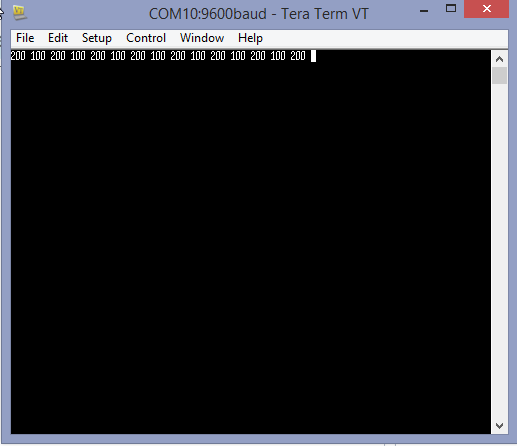
\includegraphics[scale=1] {foto1}
\newpage
\section*{Opdracht 2 b}
\begin{quote}
Als alles van onderdeel b werkt: Sluit de twee remote roudre-nodes aan op een Arduino-bordje met een XBee-shield. Laat in elk van de Arduino’s een programma draaien dat periodiek een karakter verstuurt: Bijvoorbeeld elke seconde een karakter ‘a’ door remote node 1 en elke halve seconde een ‘b’ door remote node 2. Een voorbeeldprogramma tref je aan in de bijlage 1. Alles komt dan samen op de controller. Bekijk alles via een terminalprogramma of via ‘ZigBeeOperator’. -Controleer de tijdsintervallen. -Sluit de remote Arduino-Xbee-nodes aan op een aparte voedingsspanning en leg ze elders in het lokaal neer. Ga eens na toe hoever het bereik van de nodes is.
\end{quote}
Wij hebben eerst de temperatuur sensor opgezet met de volgende code:
\begin{lstlisting}
int readingPin = A5;
int sensorValue = 0;
void setup() {
  Serial.begin(9600);
}
void loop() {
  sensorValue = analogRead(readingPin);
//To celcius 
 sensorValue *= 0.48828125;
  Serial.print(sensorValue);
  delay(10000);
}
\end{lstlisting}
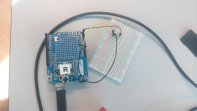
\includegraphics[scale=1] {foto2}\\
Hierna zijn we door gegaan met de coden van het writen naar de server
\\
\newpage
\begin{lstlisting}
#include <Ethernet.h>
#include <EthernetUdp.h>
#include <Dns.h>
#include <time.h>
#include <SPI.h>

int incomingByte = 0;
char buffer[20];
const int dezeMeetopstelling = 1;
//178.62.191.231
IPAddress restServer(178, 62, 191, 231); //Backup
String restServerString = "178.62.191.231";
String restServerPort   = "8080";
byte mac[] =
{
	0xDE, 0xAD, 0xBE, 0xEF, 0xFE, 0xED
};


void setup() {
	Serial.begin(9600);
	Serial.println("Programme started");
	if (Ethernet.begin(mac) == 0)
	{
		Serial.println("Failed to configure Ethernet using DHCP");
        // no point in carrying on, so do nothing forevermore:
        for (;;);
    }
    else
    {
    	Serial.print("Eth info \n Local IP: ");
    	Serial.println(Ethernet.localIP());
    	Serial.print("Subnet Mask: ");
    	Serial.println(Ethernet.subnetMask());
    	Serial.print("Gateway: ");
    	Serial.println(Ethernet.gatewayIP());
    	Serial.print("Primary DNS: ");
    	Serial.println(Ethernet.dnsServerIP());
    }
    DNSClient client;
    client.begin(Ethernet.dnsServerIP());
    if (client.getHostByName("zaku2.com", restServer) == 1)
    {
    	Serial.print("resolved server to ");
    	Serial.print(restServer);
    }
    else
    {
    	Serial.print("Unable to resolve IP, using default: ");
    	Serial.println(restServer);
    }
}

void send_pack(int number)
{
	Serial.println("send_pack");
	int contentLength;

	EthernetClient client;

	String jsonBody = String("{ \"meetopstellingen\": \""+String(dezeMeetopstelling)+"\","
	//+"\"timestamp\": "+time.year()+"-"+time.month()+"-"+time.day()+" "+time.hour()+":"+time.minute()+":"+time.second() +"\","
	+"\"waarde\": \"" + String(number)+"\"}");

	if(client.connect(restServer,8080))
	{
		client.print("POST /iws/data HTTP/1.1");
        // client.println("GET /api/newdeveloper/lights/4 HTTP/1.1");
        client.print("Host: ");
        client.print(String(restServerString+":"+restServerPort));
        client.print("Connection: keep-alive"); 
        client.print("Content-Type:   application/json; charset=UTF-8"); 
        client.print("Content-Length: "); 
        client.print(jsonBody.length());
        client.print(""); 
        client.print(jsonBody);
        client.print(""); 

        Serial.print("Sent package with body");
        Serial.print(jsonBody);       
        Serial.print(" and length ");
        Serial.println(jsonBody.length());

        while (!client.available())
        {
        	delay(1);
        }
        while (client.available()) {
        	char c = client.read();
        	Serial.print(c);
        }
    }
    else
    {
    	Serial.println("Can\'t connect");
    }
}

void loop() {
	char index = 0;
	while (Serial.available() > 0) 
	{
        // read the incoming byte:
        if(Serial.available() > 0)
        buffer[index++] = Serial.read();
    }
    if(buffer[0]!=0&&index!=0)
    {
    	Serial.println("Ontvangen:");
    	Serial.println(buffer);
    	// send_pack(buffer); We still have to add something like this
		int i = 0; while (i<21){buffer[i++]=0;} //clearing the bufffer
		index = 0;
	}

	delay(1000);
}
\end{lstlisting}
\end{document}
